\section{设计方案}
\subsection{总体设计思路}
\textcolor{black}{本次硬件设计主要设计和完善了一个可以基于 AXI 总线协议运行的 SOC 系统。其中,系统内存 (Ram)、外设 (Confreg), 以及负责管理和仲裁上述从设备与处理器间的数据交互请求, 并进行数据传输的 AXI 1X2 Bridge 模块均已在课程资料包中提供。因此, 本次设计的主要目标是构建一个支持 AXI 协议的 MIPS32 架构的 CPU, 即下图1中的mycpu\_top模块。}
\begin{figure}
	\centering
	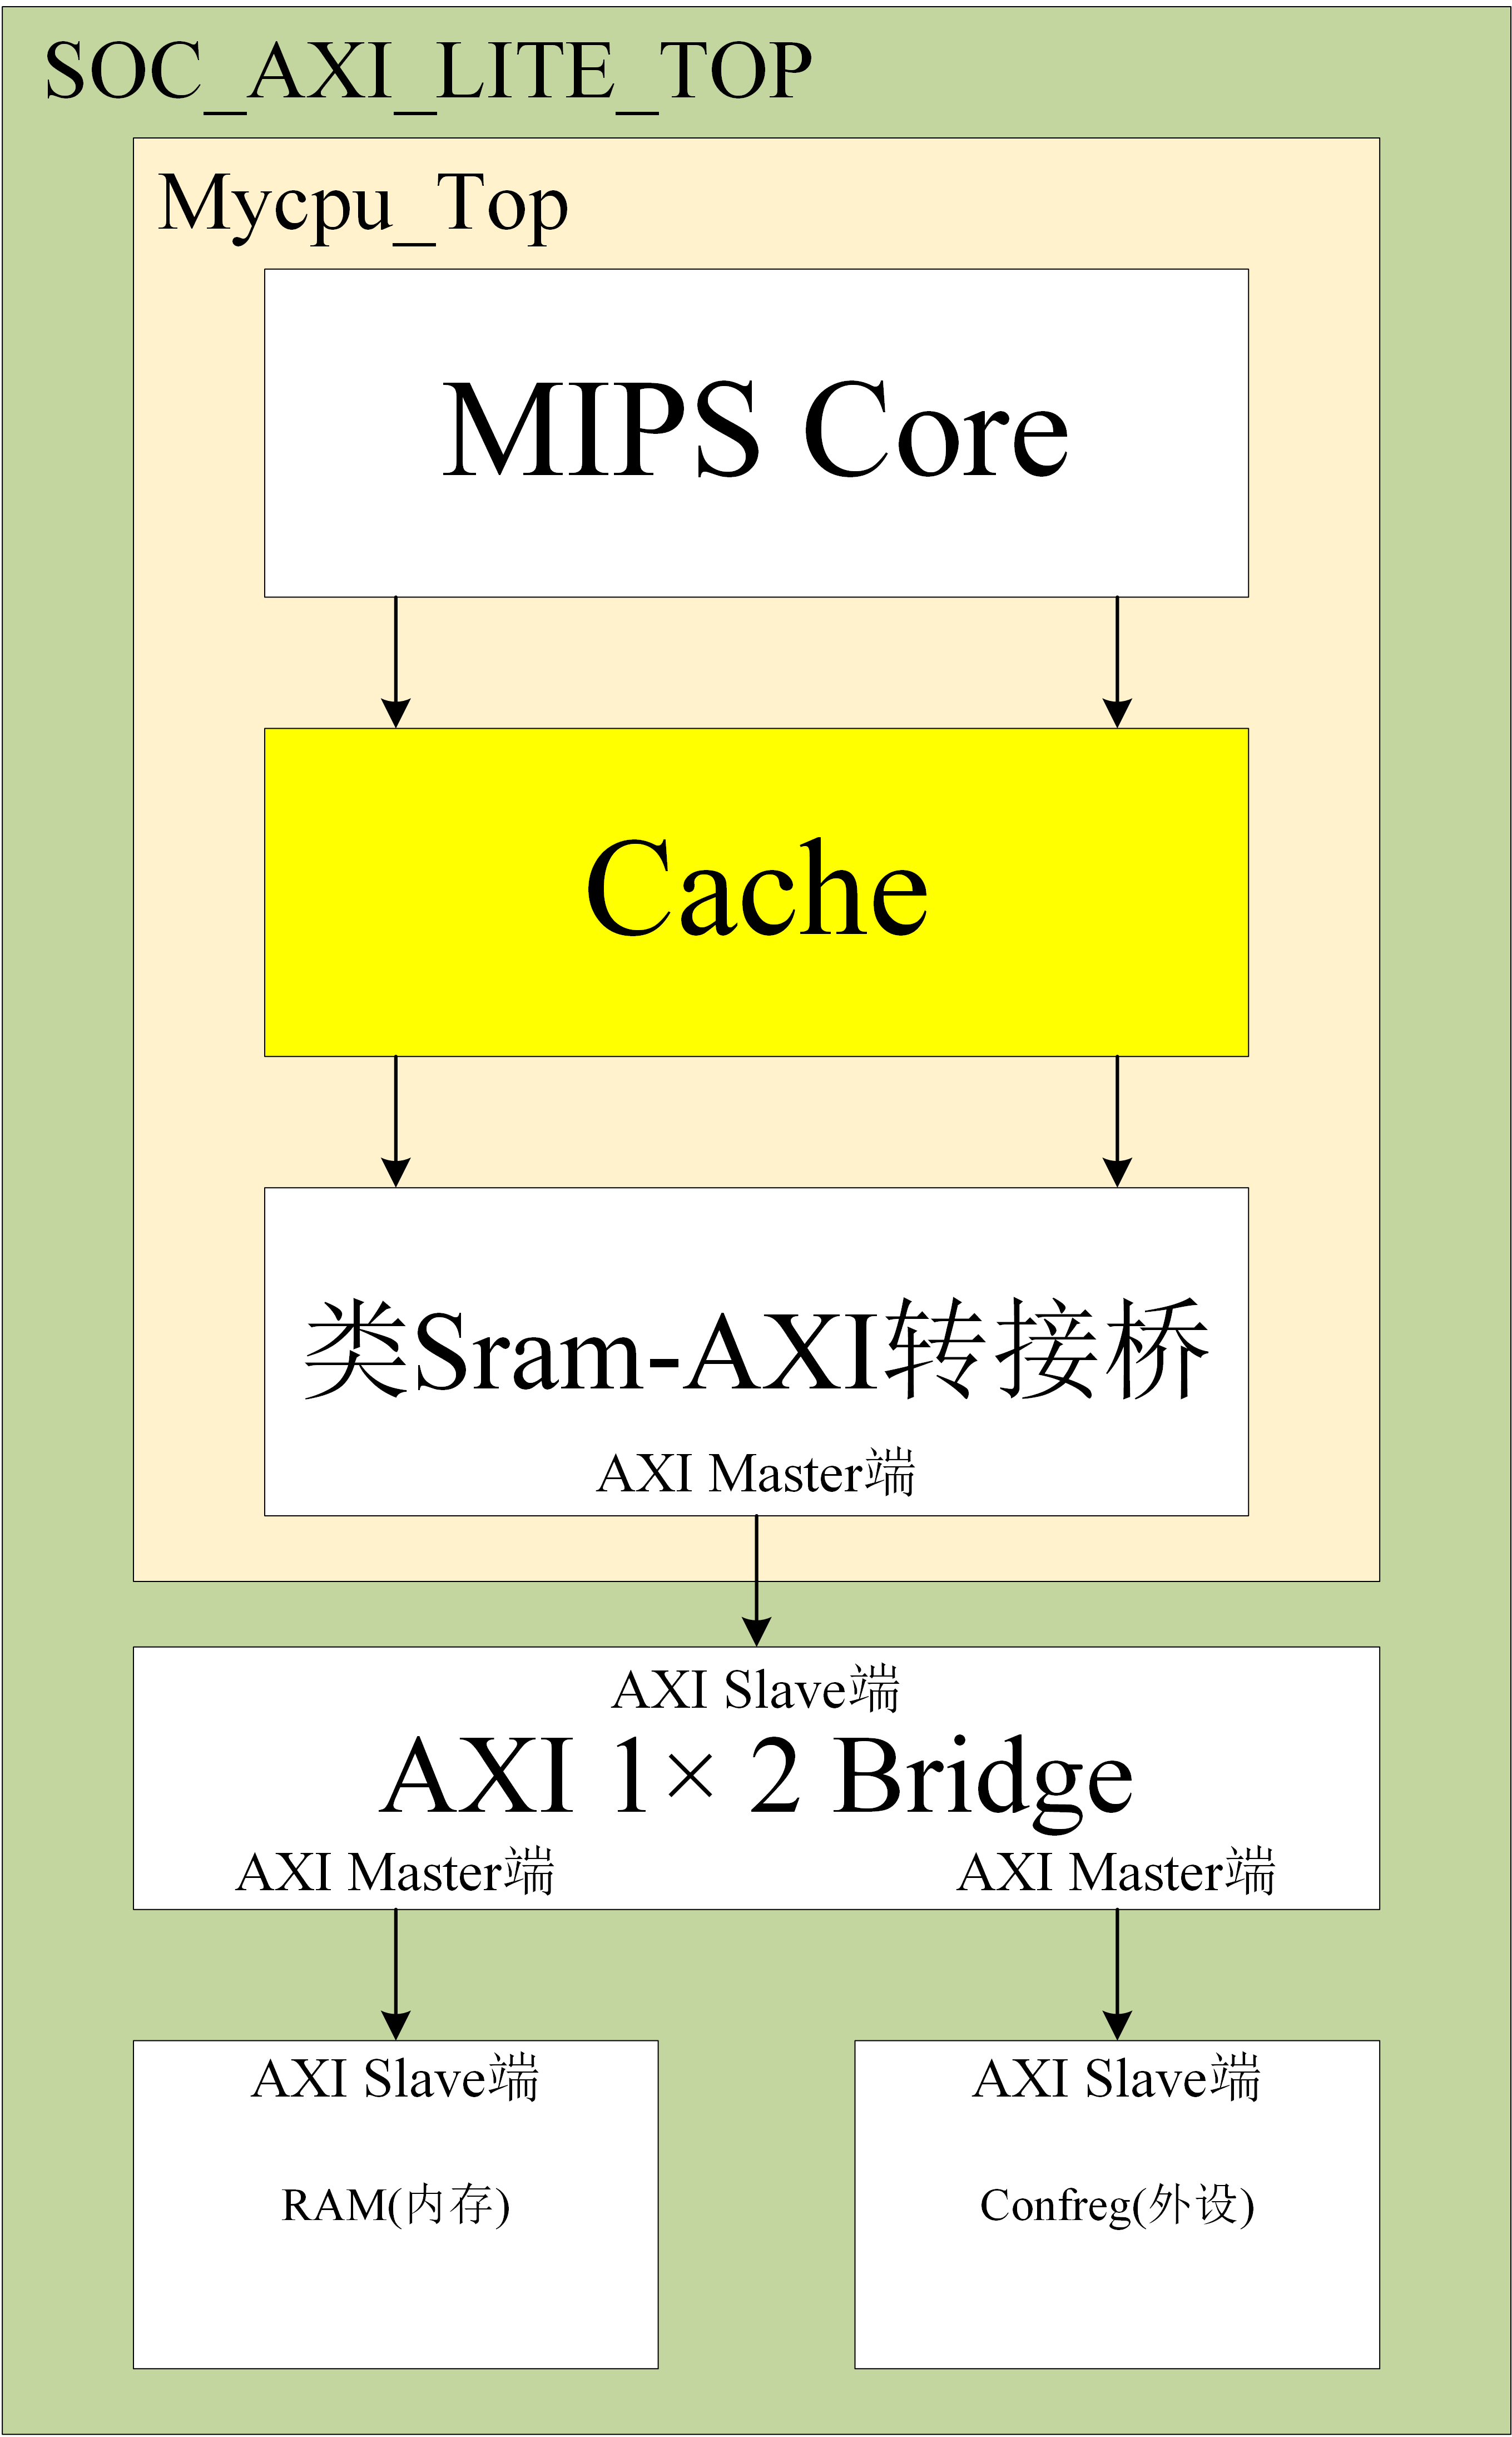
\includegraphics[width=0.5\linewidth]{image/p14.png}
	\caption{SOC顶层结构图}
	\label{fig:enter-label}
\end{figure}

本项目设计的mycpu\_top主要包含以下模块组件:\\
中央处理器MIPS:在计算机组成原理实验四所实现的五级流水线CPU基础上进行拓展,实现了MIPS32指令系统中所有非浮点MIPSI指令以及MIPS32中的ERET指令,还实现了少量CP00寄存器来支持中断和系统调用功能,但未实现TLB、MMU和特权等级。\\
内存管理单元MMU:采用直接映射方式,通过读取地址高位将CPU需访问的虚拟地址转换成物理地址,并判断数据访问请求是属于内存访问还是外设访问。\\
桥Bridge 1x2:依据MMU给出的数据访问请求类型,对内存访问请求和外设访问请求进行分离或合并操作。需要注意的是,仅内存访问请求会经过数据Cache。\\
高速缓存Cache:旨在弥补CPU与内存之间的速度差异,由指令缓存InstCache和数据缓存DataCache两部分构成。\\
桥Bridge 2x1:是Bridge 1x2的逆向工程。与Bridge 1x2不同,Bridge 2x1在某一时刻可能会同时接收到数据Cache发起的内存访问请求和CPU发出的外设访问请求,其内部仲裁策略为优先处理内存访问请求。\\
AXI接口AXInterface:mycpu\_top内部采用类SRAM方式实现数据交互,所有对外的类SRAM请求均由AXI接口统一转换为AXI请求,同时AXI接口会将外层返回的数据重新转换为类SRAM格式供内层模块使用,其内部仲裁策略为优先指令访问\\。
\begin{figure}
	\centering
	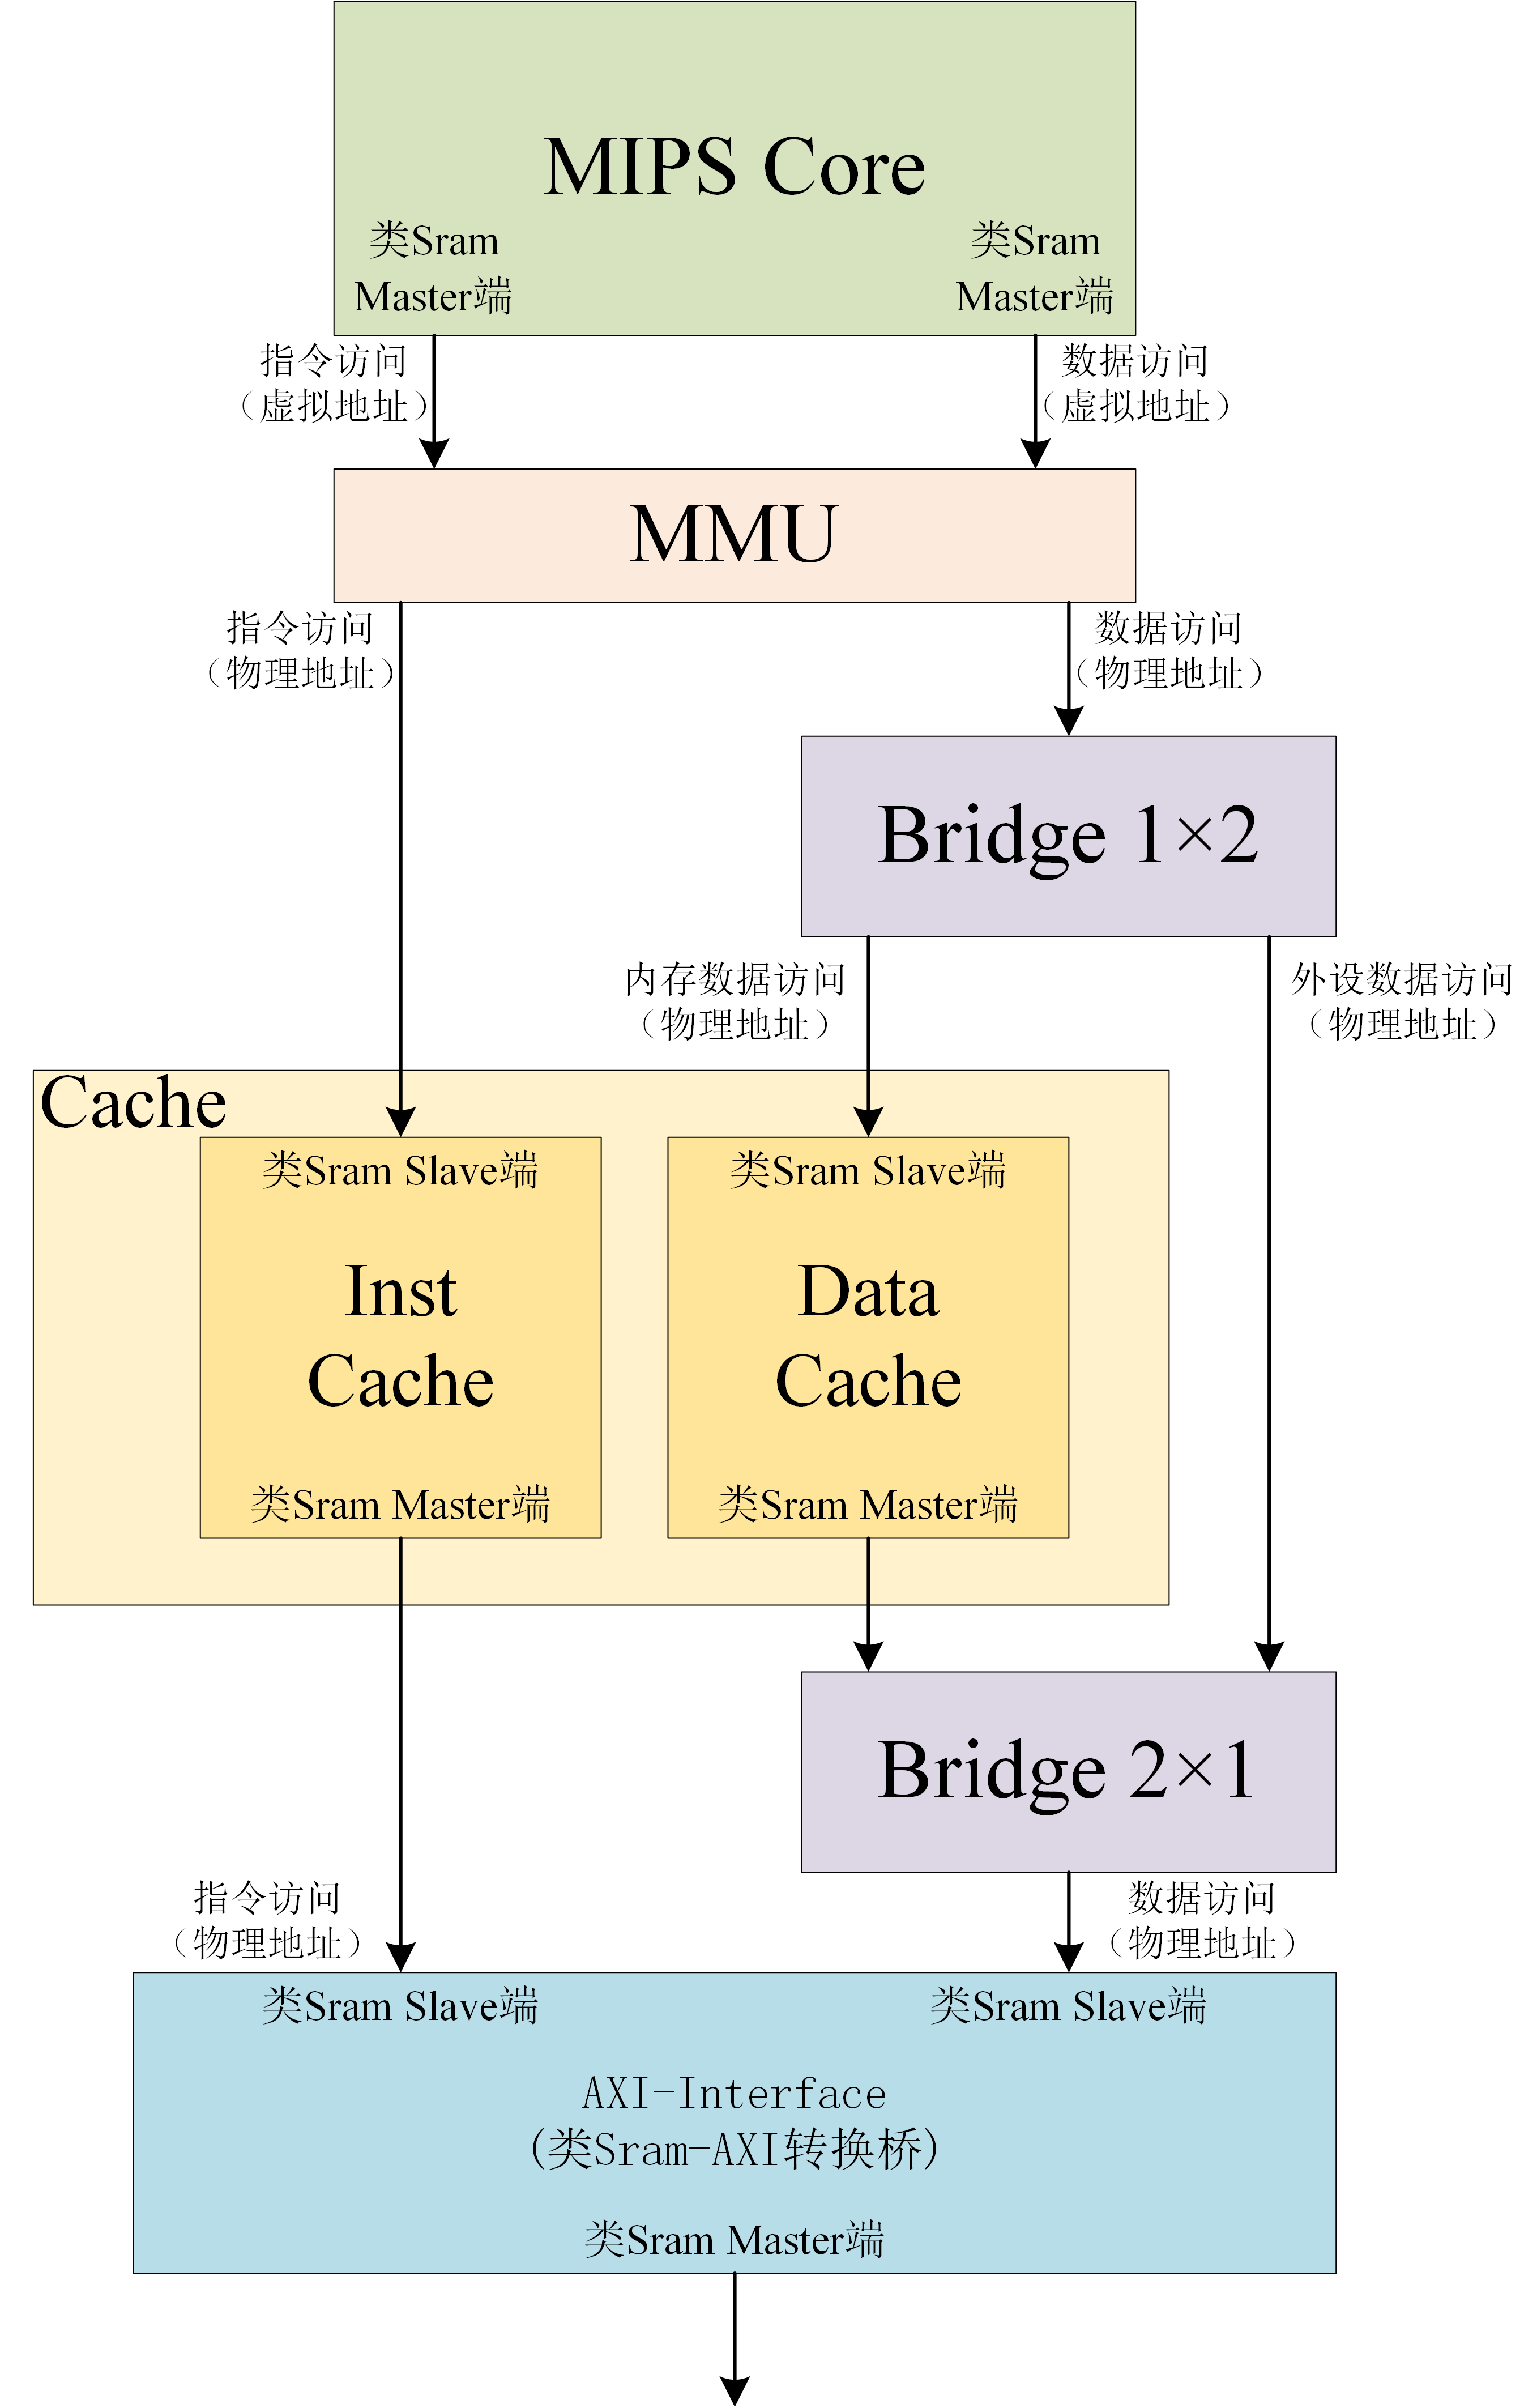
\includegraphics[width=0.5\linewidth]{image/p15.png}
	\caption{CPU顶层结构图}
	\label{fig:enter-label}
\end{figure}
\subsection{MIPS模块设计\textcolor{black}{}}

本次课程设计的核心是基于MIPS架构的五级流水线CPU。控制模块Controller、数据通路Datapath以及冒险控制模块HazardUnit在实验四时已基本搭建完成,在此次设计里需对它们进行必要的功能调整和拓展,从而确保能顺利执行前面提到的全部57条指令。类SRAM接口Sramlike是此次课程设计新引入的功能模块,其主要职责是把CPU发出的数据请求从SRAM格式转换为类SRAM格式,以便与外部模块进行更高效的数据交互。

\subsubsection{DataPath模块设计}
DatapPath作为CPU功能单元的集合,主要包括数据在各个功能部件的传输路径。而PC寄存器、寄存器堆Regfile、符号扩展与触发器 等部件无需更改,ALU仅需针对部分新增指令进行微小调整,不再此处进行赘述。因而下面将重点阐述这几个模块:DIV与HILO、Eqcmp(用于分支指令比较)、CP0与ExceptionType。

\textbf{除法器DIV}:采用采用非恢复余数除法算法 ,工作原理如下

除法器状态机:
\begin{itemize}
\item \verb|DivFree|:空闲状态,等待除法指令
\item \verb|DivOn|:正在进行除法运算
\item \verb|DivByZero|:除数为零的错误状态
\item \verb|DivEnd|:除法完成状态
\end{itemize}
除法运算过程:
\begin{itemize}
\item 初始化阶段:
\begin{itemize}
	\item 检查除数是否为0
	\item 根据\verb|signed_div_i|判断是否为有符号除法
	\item 对有符号数进行符号处理,转换为正数运算
\end{itemize}
\item 迭代计算阶段:
\begin{itemize}
	\item 使用非恢复余数除法算法
	\item 被除数左移,与除数比较
	\item 如果够减,则减去除数,商位置1
	\item 如果不够减,商位置0
	\item 重复32次得到完整商
\end{itemize}
\item 结果处理阶段:
\begin{itemize}
	\item 根据原始操作数符号恢复结果符号
	\item 商保存在低32位
	\item 余数保存在高32位
\end{itemize}
\end{itemize}

\begin{figure}
\centering
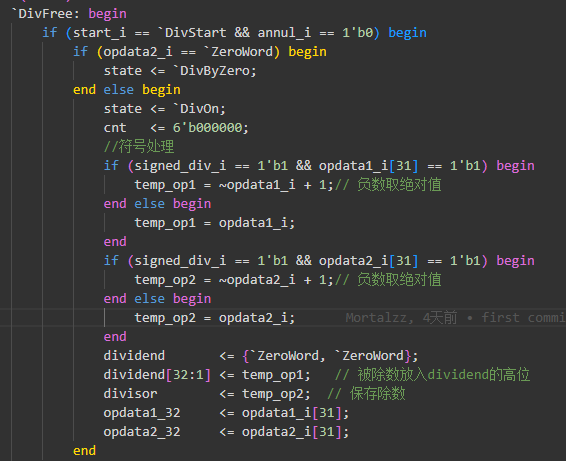
\includegraphics[width=0.5\linewidth]{image/p2.png}
\caption{DivFree状态逻辑处理}
\label{fig:enter-label}
\end{figure}

\begin{table}
\centering
\begin{tabular}{|c|c|} \hline 
	start\_i\& 开始除法运算\\ \hline 
	annul\_i\& 取消当前除法\\ \hline 
	ready\_o\& 除法完成标志\\ \hline 
	signed\_div\_i\& 有符号除法标志\\ \hline
\end{tabular}
\caption{关键控制信号}
\label{关键控制信号}
\end{table}

除法完成后,结果通过result\_o输出,在数据通路中根据hilowrite信号 将高32位(即余数)存储在HI寄存器中,将低32位(即商)存储在LO寄存器中

\begin{figure}
\centering
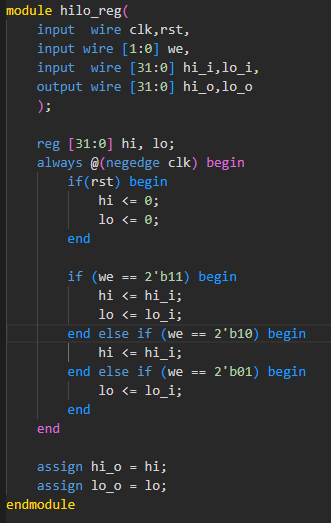
\includegraphics[width=0.5\linewidth]{image/p3.png}
\caption{HILO寄存器}
\label{fig:enter-label}
\end{figure}

\textbf{Eqcmp}:位于ID级的分支比较模块。由于在实验四中仅实现了了beq指 令,分支跳信号PCSrc当且仅当比较数A和B相等时有效。 而扩展后的57条指令中含有八条分支跳转指令,因此需要通过检测ID级指令的op和rt字段以识别指令类型 。

\begin{figure}
\centering
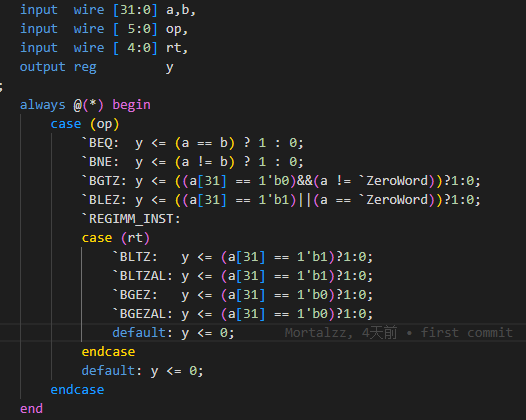
\includegraphics[width=0.5\linewidth]{image/p4.png}
\caption{Eqcmp模块}
\label{fig:enter-label}
\end{figure}

\textbf{ExceptionType模块}:MEM 级的例外处理模块,该模块负责识别CP0传入的Cause与Status寄存器值以及除中断异常外的所有异常类型,并保存错误地址、具体异常类型以及EPC以供CP0模块进行精确异常处理。 
\begin{figure}
\centering
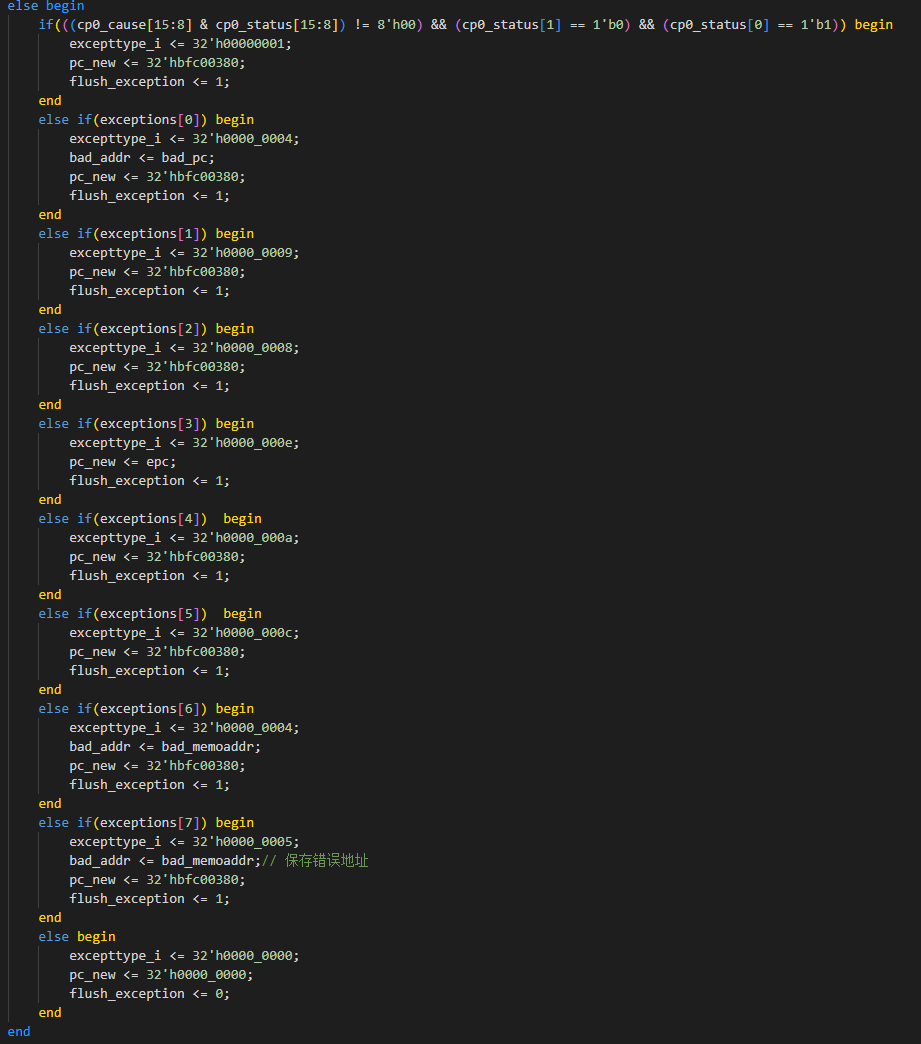
\includegraphics[width=0.5\linewidth]{image/p5.png}
\caption{异常类型判断}
\label{fig:enter-label}
\end{figure}

各异常的含义,产生的流水级和原因如下表2所示,按处理的优先级从上到下排序:


\begin{table}
\centering
\begin{tabular}{|c|c|c|c|} \hline 
	异常名称&  产生流水线&  异常描述& 异常原因\\ \hline 
	Int&  MEM&  软硬件中断&  mtc0 指令产生的软件中断或外部硬件产生的硬件中断\\ \hline 
	ADEL&  IF或MEM&  读指令或读数据异常& 地址低位与访存指令类型不匹配\\ \hline 
	ADES&  MEM&  写数据异常& 地址低位与访存指令类型不匹配\\ \hline 
	SYS&  ID&  系统调用& Syscall 指令\\ \hline 
	BP&  ID&  断点& Break 指令\\ \hline 
	REMAINDER&  ID&  保留指令& 主控制单元无法识别的指令\\ \hline 
	OV&  EX&  算术溢出& 有符号加减法结果溢出\\ \hline
	ERET& EX& 异常处理返回&Eret 指令\\\hline
\end{tabular}
\caption{异常类型及描述}
\label{tab:my_label}
\end{table}

\textbf{CP0}:位于MEM级,包含的各寄存器类型如下表3:


\begin{table}
\centering
\begin{tabular}{|c|c|} \hline 
	寄存器名称& 功能\\ \hline 
	BadVAddr& 记录最新地址相关例外(Adel或Ades)的出错地址。\\ \hline 
	Count& 处理器内部计数器。用于触发时钟中断,\\ \hline 
	Status& 处理器状态与控制寄存器。\\ \hline 
	Cause& 存放上一次例外原因。\\ \hline
	EPC&存放上一次发生例外指令的PC。\\\hline
\end{tabular}
\caption{CP0寄存器}
\label{tab:my_label}
\end{table}

\begin{figure}
\centering
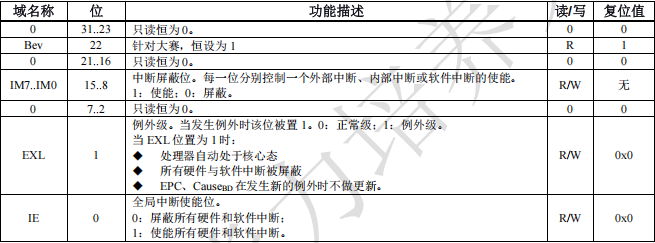
\includegraphics[width=0.5\linewidth]{image/P6.png}
\caption{Status寄存器}
\label{fig:enter-label}
\end{figure}
\begin{figure}
\centering
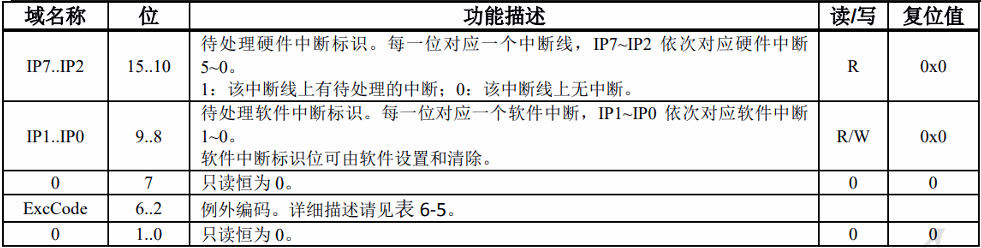
\includegraphics[width=0.5\linewidth]{image/P7.png}
\caption{Cause寄存器}
\label{fig:enter-label}
\end{figure}
各异常处理的实现流程如下:

\textbf{中断处理}:最高级别例外。本次项目设计中只实现软件中断。软件中断的产生原理为软件调用mtc0指令,该指令在MEM阶段不经过Exception模块,而是直接对Cause寄存器的对应比特位进行写操作,因此无论mtc0之后的一条指令 执行情况如何,该指令都将被认为触发了软件中断,PC寄存器将跳转至异常处理程序入口地址;特别强调,与其他异常指令的不同之处在于,触发中断异常处 理的是mtc0指令的下一条指令,而不是其本身。 

\textbf{Eret 指令的处理}: 异常处理返回。严格来说,Eret并不是一种异常,但同样需要 对CP0寄存器的状态进行部分修改,因此采用类似的处理。该异常触发时,PC 寄存器将跳转至EPC寄存器中保存的指令地址,即从异常处理程序中返回并继 续往后执行;特别强调,与其他分支跳转指令的不同之处在于,由于Eret指令理 论上是异常处理程序的最后一条指令,其延迟槽地址内存放的可能是来自其他 程序的指令,因此MEM级的Eret指令不能执行其延迟槽指令或后续的任何其 他指令。而是需要像其他异常指令一样对流水线进行彻底的刷新,以避免程序 的错误运行。 

\textbf{BadVAddr 寄存器处理}: 当且仅当异常类型为地址异常时,向BadVAddr寄存器 中写入错误地址。

\textbf{EPC寄存器处理}:当异常指令不是延迟槽指令时,EPC中写入该指令的PC地 址,以便异常处理程序返回后重现从该指令继续运行;当异常指令是延迟槽指 令时,EPC中写入的是延迟槽指令的上一条指令,即分支跳转指令的PC地址。 因为跳转后的程序在异常处理开始前尚未执行,因此异常处理完成后需要重新 从此处开始执行。 
\begin{figure}
\centering
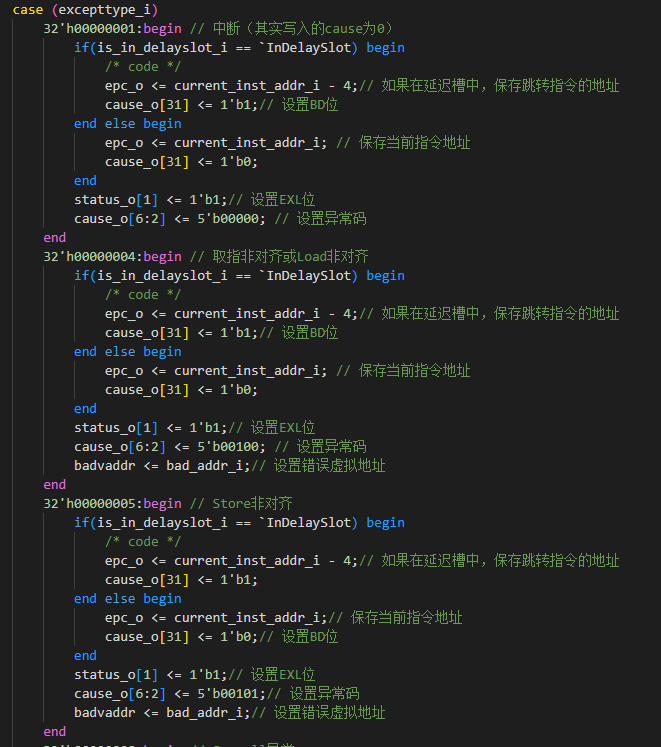
\includegraphics[width=0.5\linewidth]{image/p8.png}
\caption{部分异常处理逻辑}
\label{fig:enter-label}
\end{figure}

\subsubsection{Hazard模块设计}
冒险控制模块。该模块的大部分实现与实验四一致, 此处重点阐述需要进行修改或添加的部分。

\textbf{longest\_stall:}
这是最长暂停信号,由指令存储器、数据存储器或除法引起,当出现取址或访存指令时,我们需要暂停整个流水线,因为内存的访问时间开销大,全流水线必须阻塞,等待上述过程执行完成。同理,由于除法器需要36个CPU周期时间来完成除法运算,于是同样阻塞全流水线,等待除法过程完毕。
\begin{figure}[h]
\centering
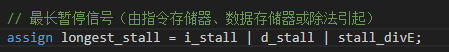
\includegraphics[width=1\linewidth]{image/hazard1.png}
\caption{最长暂停信号}
\label{fig:enter-label}
\end{figure}

\begin{figure}[h]
\centering
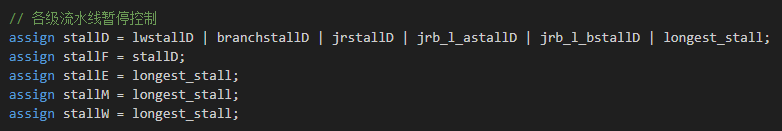
\includegraphics[width=1\linewidth]{image/hazard2.png}
\caption{流水线暂停逻辑}
\label{fig:enter-label}
\end{figure}

\textbf{ForwardaE\&ForwardbE:}
这是执行级前推信号,用于ALU运算.代码通过两个2位的控制信号forwardaE和forwardbE来控制数据前推。当执行阶段的指令需要使用之前指令的结果时,系统会检查源寄存器号(rsE和rtE)是否与访存阶段(M)或写回阶段(W)的目标寄存器号匹配。如果匹配且对应阶段的寄存器写使能信号有效,就会触发相应的数据前推。具体来说,如果与访存阶段匹配,则设置前推信号为2'b10;如果与写回阶段匹配,则设置为2'b01。这种机制优先从访存阶段前推,其次是写回阶段,并且只有当源寄存器号不为0时才进行前推(因为0号寄存器永远为0)。
\begin{figure}[h]
\centering
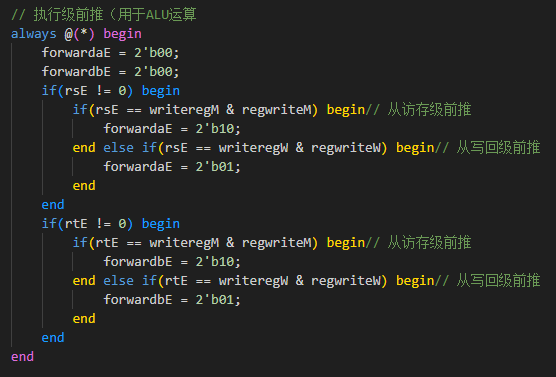
\includegraphics[width=0.5\linewidth]{image/hazard3.png}
\caption{执行级数据前推}
\label{fig:enter-label}
\end{figure}

\textbf{ForwardaD\&ForwardbD:}
这是译码级数据前推信号,用于分支判断.代码通过两个1位的控制信号forwardaD和forwardbD来控制数据前推。当译码阶段的分支判断需要使用之前指令的结果时,系统会检查源寄存器号(rsE和rtE)是否与访存阶段(M)的目标寄存器号匹配。如果匹配且对应阶段的寄存器写使能信号有效,就会触发相应的数据前推。具体来说,如果匹配,则设置前推信号为1'b1。
\begin{figure}[h]
\centering
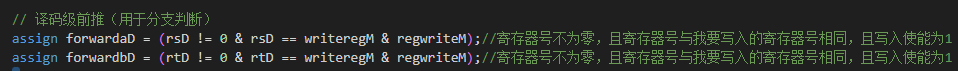
\includegraphics[width=1\linewidth]{image/hazard9.png}
\caption{译码级数据前推}
\label{fig:enter-label}
\end{figure}

\textbf{forwardhiloE:}
该信号用于实现HI/LO寄存器的数据前推逻辑,主要用于处理乘除法指令的结果前推。当执行阶段的指令是MFHI(从HI寄存器读取)或MFLO(从LO寄存器读取)指令时(由alucontrolE信号判断),系统会检查访存阶段和写回阶段是否有对HI/LO寄存器的写操作(通过hilo\_weM和hilo\_weW信号判断)。如果访存阶段有HI/LO寄存器写操作,则设置前推信号forwardhiloE为2'b10进行访存级前推;如果写回阶段有HI/LO寄存器写操作,则设置为2'b01进行写回级前推。
\begin{figure}[h]
\centering
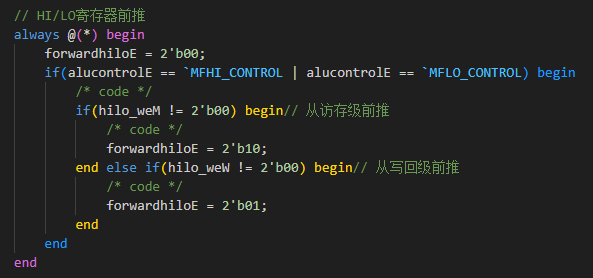
\includegraphics[width=1\linewidth]{image/hazard4.png}
\caption{HI/LO寄存器数据前推}
\label{fig:enter-label}
\end{figure}

\newpage
\textbf{lwstallD:}
用于标记lw与sw指令后的数据冒险,使得D与F阶段流水线暂停以等待数据就绪
\begin{figure}[h]
\centering
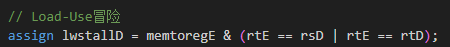
\includegraphics[width=1\linewidth]{image/hazard5.png}
\caption{Load-use数据冒险}
\label{fig:enter-label}
\end{figure}

\textbf{jrstallD:}
用于标记寄存器跳转时的出现的寄存器跳转冒险,使得D与F阶段流水线暂停以等待数据就绪
\begin{figure}[h]
\centering
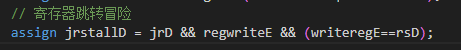
\includegraphics[width=1\linewidth]{image/hazard6.png}
\caption{寄存器跳转冒险}
\label{fig:enter-label}
\end{figure}

\textbf{branchstallD:}
实现分支指令的数据冒险检测逻辑,通过branchstallD信号来判断当前译码阶段的分支指令(branchD)是否依赖于前面指令的运算结果:如果执行阶段有写寄存器操作(regwriteE)或访存阶段有访存写寄存器操作(memtoregM),且这些指令的目标寄存器(writeregE或writeregM)与分支指令的源操作数寄存器(rsD或rtD)相匹配,则需要产生流水线停顿信号以等待数据就绪。
\begin{figure}[h]
\centering
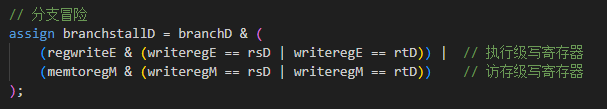
\includegraphics[width=1\linewidth]{image/hazard10.png}
\caption{分支冒险}
\label{fig:enter-label}
\end{figure}

\newpage
\textbf{jrb\_l\_astallD\&jrb\_l\_bstallD:}
实现Load指令后跟跳转/分支指令时的冒险检测逻辑,通过jrb\_l\_astallD和jrb\_l\_bstallD信号来检测当前译码阶段的跳转/分支指令(jrD|branchD)是否依赖于前面执行阶段或访存阶段的Load指令的结果(由memtoregE和memtoregM表示),其中分别检查源寄存器rsD和rtD是否与Load指令的目标寄存器(writeregE或writeregM)相匹配,如果匹配则需要流水线停顿以等待Load指令完成。
\begin{figure}[h]
\centering
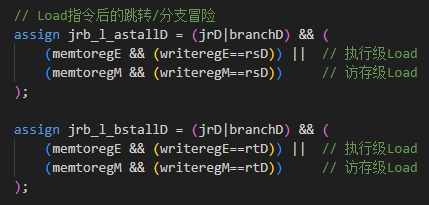
\includegraphics[width=1\linewidth]{image/hazard7.png}
\caption{Load指令后的跳转/分支冒险}
\label{fig:enter-label}
\end{figure}

\textbf{flush\_x:}
因异常引起的流水线刷新逻辑,通过flushF、flushD、flushE、flushM和flushW信号来控制不同阶段的流水线刷新;当在访存阶段发生异常(flush\_exceptionM不为0)时,取指令阶段(F)、译码阶段(D)、访存阶段(M)和写回阶段(W)都会被刷新,而在执行阶段(E)则在发生Load指令数据冒险、分支指令数据冒险或Load指令后跟跳转/分支指令时(且不处于最长暂停状态)也会触发刷新,这样可以确保在异常发生时流水线中的指令能够被正确处理,避免错误执行。
\begin{figure}[h]
\centering
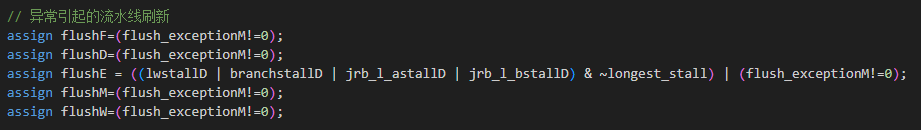
\includegraphics[width=1\linewidth]{image/hazard8.png}
\caption{异常引起的流水线刷新}
\label{fig:enter-label}
\end{figure}

\subsubsection{Controller模块设计}

CPU的主控制单元,包含主控制译码器Maindec、ALU控制译码器Aludec以及流水线寄 存器的控制信号部分,整体架构与实验四中完全一致。在此基础上,添加了若干新的控制信号,并对流水线进行了相应调整。由于Aludec和流水线寄存器的工作过程相较于实验 四基本没有变化,只是简单的堆砌新的对应关系,因此不再赘述。此处重点阐述Maindec 模块所产生的各控制信号含义及其解析过程。 


\begin{table}[h]
\centering
\begin{tabular}{|c|c|c|} \hline 
	信号名&  位宽& 功能描述\\ \hline 
	regwrite&  1-bit& 写寄存器堆\\ \hline 
	regdst&  1-bit& 目的寄存器号来源,0->Rt字段,1->Rd字段\\ \hline 
	alusrc&  1-bit& 第二个ALU操作数源,0-> 第二个寄存器堆输出,1->
	立即数符号扩展\\ \hline 
	memtoreg&  1-bit& 内存到寄存器的数据选择信号,决定写回寄存器的数据是来自内存还是ALU结果\\ \hline 
	extop&  1-bit& 立即数扩展方式选择信号,控制立即数是进行符号扩展还是零扩展\\ \hline 
	hilo\_we&  2-bit& HI、LO寄存器写使能信号,用于乘除法运算结果的存储\\ \hline 
	branch&  1-bit& 分支指令控制信号,表示当前指令是否为分支指令\\ \hline 
	jump&  1-bit& 跳转指令控制信号,表示当前指令是否为跳转指令\\ \hline 
	jr&  1-bit& 寄存器跳转控制信号,用于jr(跳转到寄存器)类指令\\ \hline 
	al& 1-bit&链接跳转控制信号,用于需要保存返回地址的跳转指令\\ \hline 
	jalr& 1-bit&寄存器链接跳转控制信号,用于jalr指令\\ \hline 
	cp0\_we& 1-bit&CP0协处理器写使能信号\\ \hline 
	cp0\_re& 1-bit&CP0协处理器读使能信号\\ \hline 
	invaild& 1-bit&非法指令标志,表示当前指令是否为非法指令\\ \hline 
	aluiop& 4-bit&ALU操作码,控制ALU执行什么样的运算\\ \hline
\end{tabular}
\caption{控制信号定义}
\label{tab:my_label}
\end{table}

其中需要重点说明的有hilo\_we、jalr、cp0\_we、cp0\_re以及invaild信号。


hilo\_we(HILO寄存器写使能) 作用:

\begin{itemize}
\item 控制HILO寄存器的写入操作
\item 用于乘除法指令的结果存储
\end{itemize}
工作过程:

\begin{itemize}
\item 乘法指令(MULT/MULTU)执行时置1,结果写入HI、LO
\item 除法指令(DIV/DIVU)执行时置1,商写入LO,余数写入HI
\item MTHI/MTLO指令执行时置1,直接写入对应寄存器
\item 其他指令时置0,保护HILO寄存器内容
\end{itemize}

jalr(寄存器跳转并链接) 作用:

\begin{itemize}
\item 控制寄存器跳转并保存返回地址
\item 实现函数调用和返回机制
\end{itemize}
工作过程:

\begin{itemize}
\item JALR指令执行时置1
\item 将当前PC+8保存到指定寄存器(通常是\$ra)
\item 跳转到寄存器中指定的地址
\item 支持嵌套函数调用
\end{itemize}

cp0\_we(CP0寄存器写使能) 作用:

\begin{itemize}
\item 控制CP0协处理器寄存器的写入
\item 用于系统控制和异常处理
\end{itemize}
工作过程:

\begin{itemize}
\item MTC0指令执行时置1
\item 允许写入指定的CP0寄存器
\item 用于修改系统状态、中断控制等
\item 特权指令,只能在内核模式执行
\end{itemize}

cp0\_re(CP0寄存器读使能) 作用:

\begin{itemize}
\item 控制CP0协处理器寄存器的读取
\item 获取系统状态和异常信息
\end{itemize}
工作过程:

\begin{itemize}
\item MFC0指令执行时置1
\item 允许读取指定的CP0寄存器内容
\item 用于查询系统状态、获取异常信息
\item 特权指令,只能在内核模式执行
\end{itemize}

invalid(无效指令标志) 作用:

\begin{itemize}
\item 标识当前指令是否为有效的MIPS指令
\item 触发无效指令异常
\end{itemize}
工作过程:

\begin{itemize}
\item 指令译码时检查操作码和功能码
\item 遇到未定义指令时置1
\item 触发无效指令异常(Reserved Instruction Exception)
\item 跳转到异常处理程序

\end{itemize}


\begin{figure}
\centering
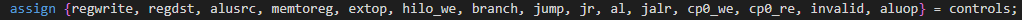
\includegraphics[width=0.5\linewidth]{image/p9.png}
\caption{控制信号赋值}
\label{fig:enter-label}
\end{figure}

\begin{figure}
\centering
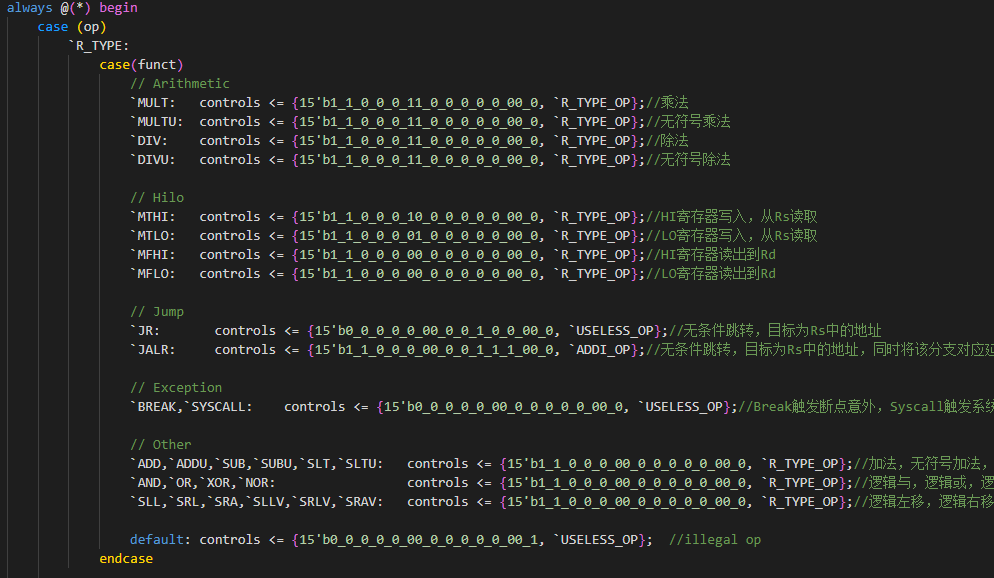
\includegraphics[width=0.5\linewidth]{image/p10.png}
\caption{控制信号赋值}
\label{fig:enter-label}
\end{figure}

\subsubsection{Sram\_Like模块设计}
总体功能:
\begin{itemize}
\item 将同步SRAM接口转换为握手协议的SRAM-Like接口
\item 处理指令和数据访问的时序要求
\item 实现CPU与存储系统的高效通信
\end{itemize}

i\_sram\_to\_sram\_like(指令接口转换):

主要功能:

\begin{itemize}
\item 处理指令获取请求
\item 实现指令读取的握手协议
\item 管理指令缓存访问
\end{itemize}
工作过程:

\begin{enumerate}
\item 请求阶段:
\begin{itemize}
	\item 接收CPU发出的指令读取请求
	\item 生成SRAM-Like接口所需的控制信号
	\item 发送地址和控制信息
\end{itemize}
\item 等待阶段:
\begin{itemize}
	\item 等待存储系统的响应
	\item 处理addr\_ok信号(地址接收确认)
	\item 处理data\_ok信号(数据有效确认)
\end{itemize}
\item 完成阶段:
\begin{itemize}
	\item 接收指令数据
	\item 向CPU传递读取的指令
	\item 完成本次指令获取
\end{itemize}
\item d\_sram\_to\_sram\_like(数据接口转换):
\end{enumerate}
主要功能:

\begin{itemize}
\item 处理数据读写请求
\item 实现数据访问的握手协议
\item 管理数据缓存访问
\end{itemize}
工作过程:

\begin{enumerate}
\item 读请求处理:
\begin{itemize}
	\item 接收CPU的数据读取请求
	\item 转换为SRAM-Like读请求
	\item 处理不同数据宽度(字/半字/字节)
\end{itemize}
\item 写请求处理:
\begin{itemize}
	\item 接收CPU的数据写入请求
	\item 生成写使能信号
	\item 处理写数据对齐
\end{itemize}
\item 握手控制:
\begin{itemize}
	\item 管理addr\_ok信号
	\item 管理data\_ok信号
	\item 控制数据传输时序
\end{itemize}
\item 关键特性:i\_sram\_to\_sram\_like与d\_sram\_to\_sram\_like的共同点在于都采用了握手协议以实现可靠传输以及采用缓冲机制以处理速度不匹配问题。但d\_sram需要处理读写操作,更复杂
\end{enumerate}
%\end{itemize}
\begin{figure}
\centering
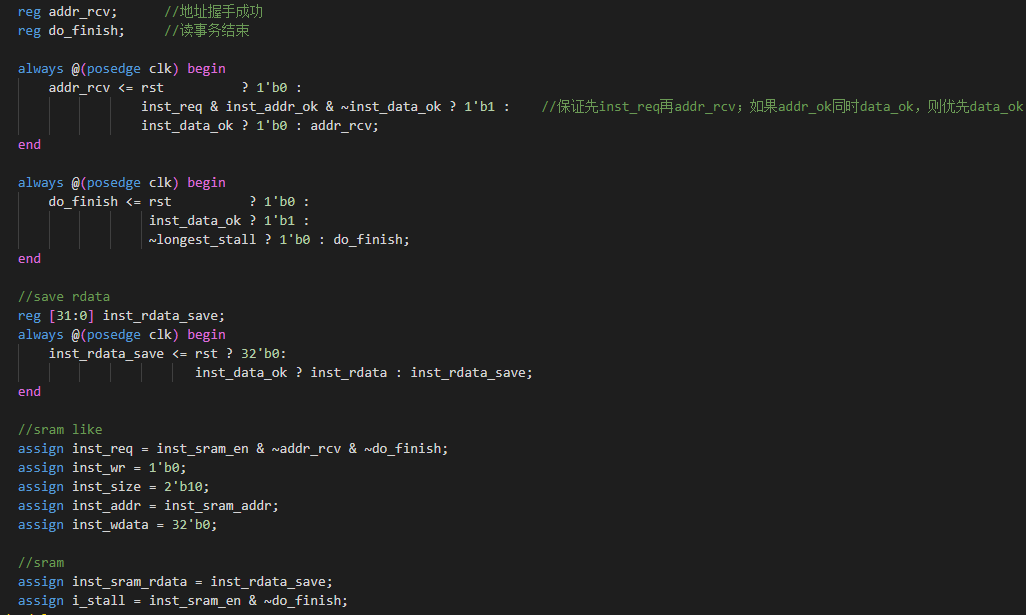
\includegraphics[width=0.5\linewidth]{image/P11.png}
\caption{isram}
\label{fig:enter-label}
\end{figure}
\begin{figure}
\centering
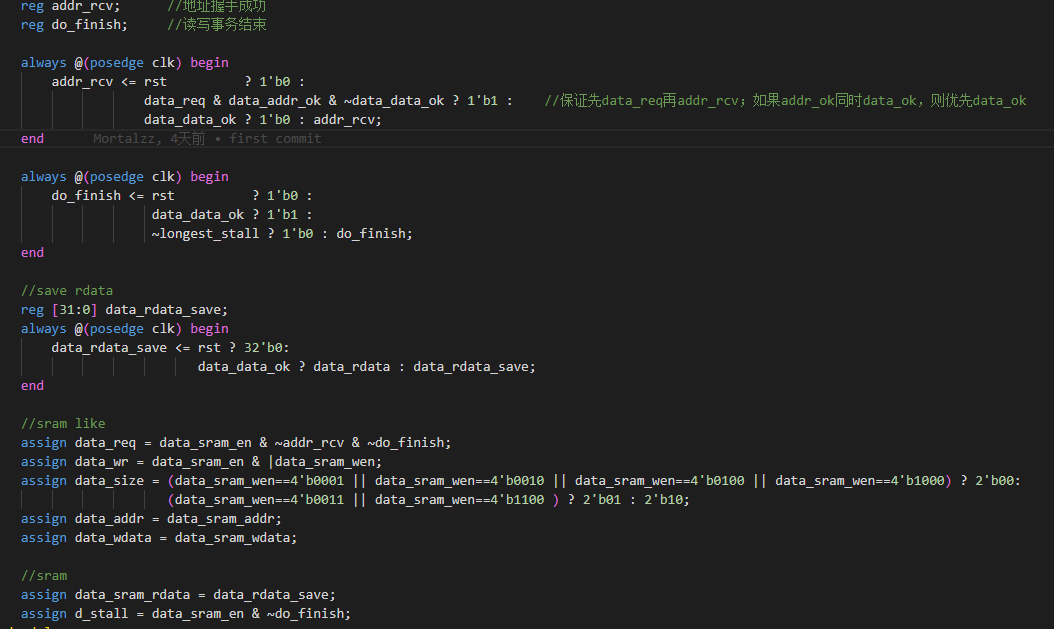
\includegraphics[width=0.5\linewidth]{image/P12.png}
\caption{dsram}
\label{fig:enter-label}
\end{figure}


\begin{flushleft}
\subsection{Bridge模块设计}
\subsubsection{Bridge1x2模块设计}
基于now\_dcache 信号区分数据请求,两类请求不会同时产生,不涉及仲裁逻辑。
\end{flushleft}

\begin{flushleft}
\subsubsection{Bridge 2x1 模块设计}
用于仲裁两个Cache端口的访问请求,将两个Cache接口服用到一个AXI接口,保证了访问的公平性和正确性,这里的优先级控制采用了固定优先级策略,规定数据Cache优先级高于指令Cache,从而避免了数据相关导致的死锁,工作流程如下:
\end{flushleft}
\begin{flushleft}
a)请求仲裁:
\begin{itemize}
\item 检测两个Cache的请求信号
\item 根据优先级选择服务对象
\item 生成仲裁结果信号
\end{itemize}

b) 数据传输:
\begin{itemize}
\item 连接选中的Cache到AXI接口
\item 传递地址和控制信号
\item 管理数据流向
\end{itemize}

c) 完成处理:
\begin{itemize}
\item 等待当前传输完成
\item 释放总线资源
\item 准备下一次仲裁
\end{itemize}
\end{flushleft}

\begin{figure}
\centering
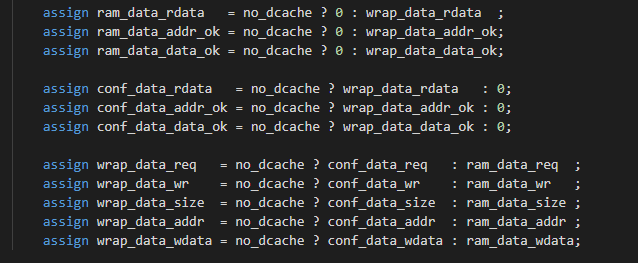
\includegraphics[width=0.5\linewidth]{image/p13.png}
\caption{Bridge2x1模块}
\label{fig:enter-label}
\end{figure}
\begin{flushleft}
\subsection{ Cache设计}
\subsubsection{DCache设计}

\subsubsection{ICache设计}
\end{flushleft}



\begin{flushleft}
\subsection{AXInterface模块设计}
对来自InstCache 的取指请求和来自Bridge2x1的访存请求进行仲裁,并转换为AXI格式。仲裁逻辑为指令请求优先。本次项目设计使用的是参考资料包中提供的类 ,因此不在此处过多解释。
\end{flushleft}
